\begin{figure}
\centering
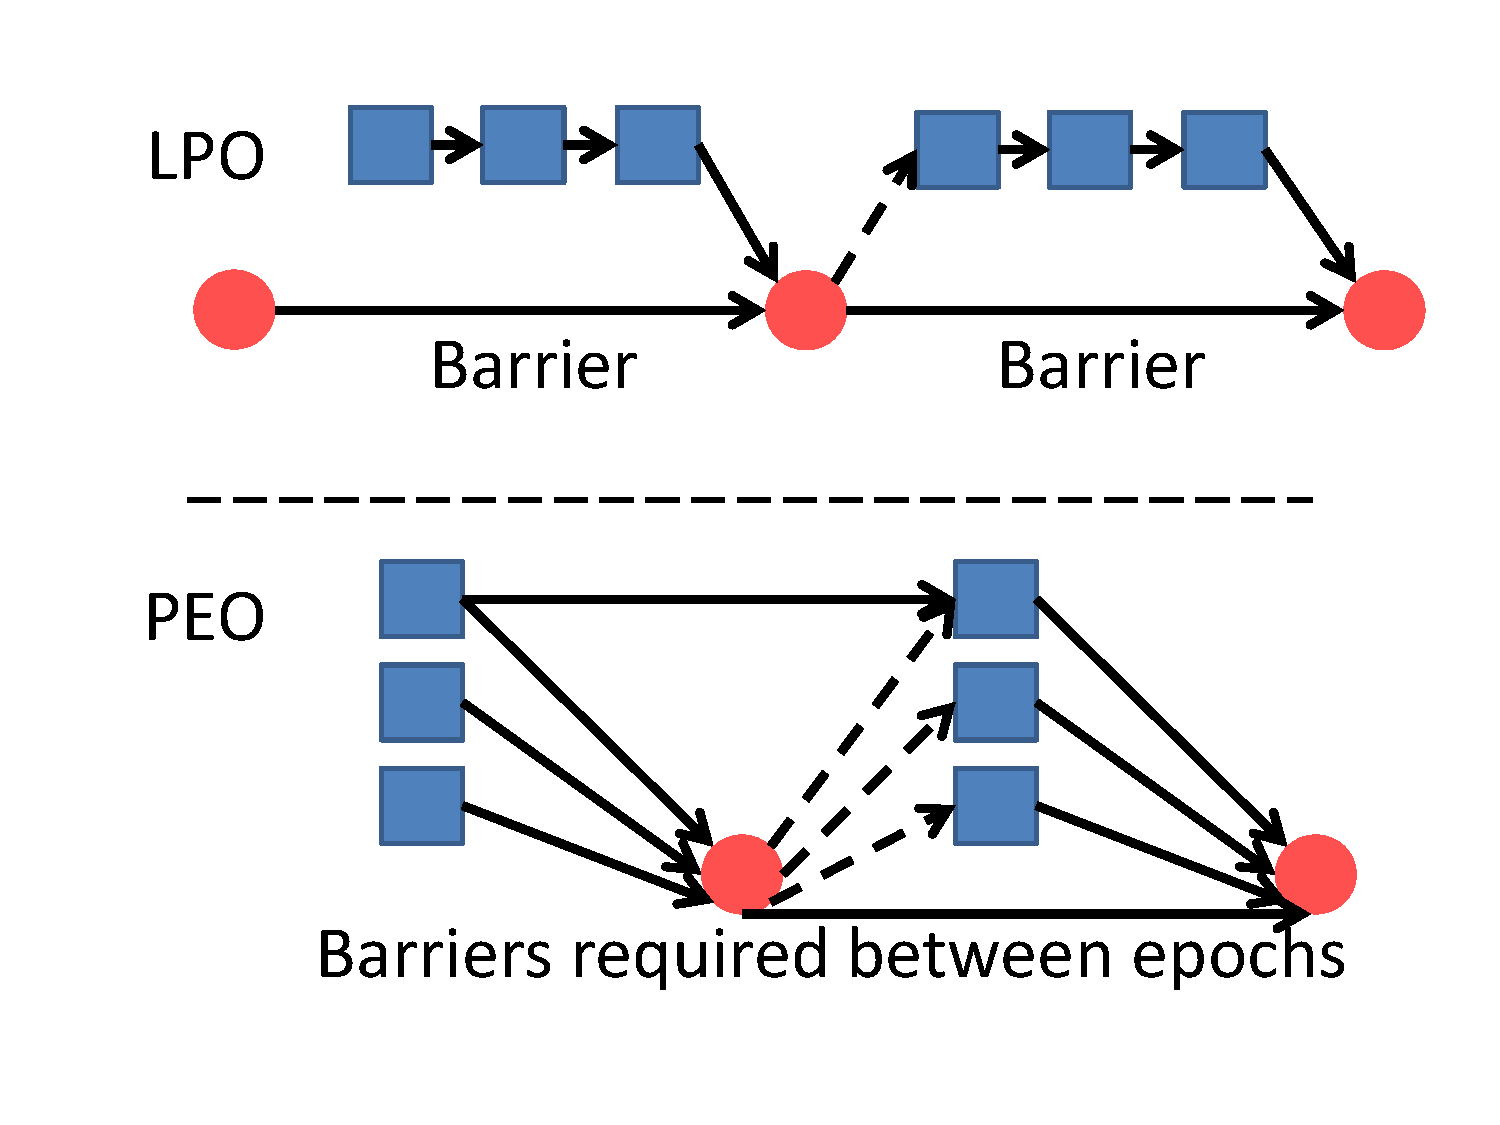
\includegraphics[width=\textwidth]{PMC_patterns/buffer_PEO_LPO.pdf}
\caption{Buffer execution under LPO and PEO.  LPO (top) removes persist dependencies between persisting the counter value and subsequent buffer persists.  Such dependencies still remain when adjacent buffer inserts are from the same thread.  Atomic persist segments within each buffer persist serialize.  PEO (bottom) allows buffer data to persist in parallel.  Buffer data necessarily persists before counter data for correctness, but counter values additionally persist before subsequent buffer persists, even from remote threads.}
\label{figure::buffer_PEO_LPO}
\end{figure}
